\section{Link Layer -- Media Access and Switching}
\subsection{Wired Media Access}
\begin{figure}[H]
    \tikzsetnextfilename{wired-media-access}
    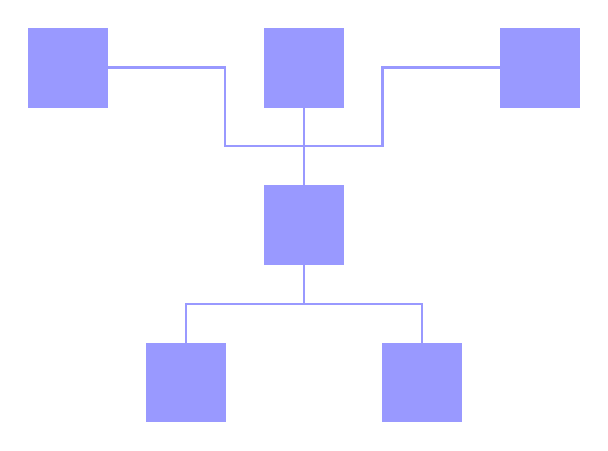
\begin{tikzpicture}[every node/.style={draw,blue!40!white,fill,rectangle,minimum width=1cm,minimum height=1cm}]
        \node at (0,0) (1) {};
        \node at (3,0) (2) {};
        \node at (6,0) (3) {};
        \node at (3,-2) (4) {};
        \node at (1.5,-4) (5) {};
        \node at (4.5,-4) (6) {};
        \draw[blue!40!white,thick] (1) -| (2,-1) -- (4,-1) |- (3);
        \draw[blue!40!white,thick] (2) -- (4) -- (3,-3);
        \draw[blue!40!white,thick] (5) |- (3,-3);
        \draw[blue!40!white,thick] (6) |- (3,-3);
    \end{tikzpicture}
\end{figure}

\subsection{Link Layer}
\begin{itemize}[nosep]
    \item Single-hop addressing
    \item Media Access
    \item Single-hop reliability
\end{itemize}

\subsection{Media Access Control}
\begin{itemize}[nosep]
    \item Control access to shared physical medium
          \begin{itemize}[nosep]
              \item e.g. who can talk when?
              \item If everyone talks at once, no one hears anything
              \item Job of the Link Layer
          \end{itemize}
    \item Two conflicting goals
          \begin{itemize}[nosep]
              \item Maximize utilization when one node sending
              \item Aproach $\sfrac{1}{n}$ when $n$ nodes sending
          \end{itemize}
\end{itemize}

\subsection{Different Approaches}
\begin{itemize}[nosep]
    \item Partitioned Access
          \begin{itemize}[nosep]
              \item Time Division Multiple Access (TDMA)
              \item Frequency Division Multiple Access (FDMA)
              \item Code Division Multiple Access (CDMA)
          \end{itemize}
    \item Random Access
          \begin{itemize}[nosep]
              \item ALOHA/Slotted ALOHA
              \item Carrier Sense Multiple Access/Collision Detection (CSMA/CD)
              \item Carrier Sense Multiple Access/Collision Avoidance (CSMA/CA)
              \item RTS/CTS (Request to Send/Clear to Send)
              \item Token-based
          \end{itemize}
\end{itemize}

\subsection{Collision Detection}
\begin{itemize}[nosep]
    \item Without minimum frame length, might not detect collision
\end{itemize}
\subsection{Case Study: Ethernet (802.3)}
\begin{itemize}[nosep]
    \item Dominant wired LAN technology
    \item Both Physical and Link Layer specification
    \item CSMA/CD
          \begin{itemize}[nosep]
              \item Carrier Sense / Multiple Access / Collision Detection
          \end{itemize}
    \item Frame Format (Manchester Encoding):
          \begin{figure}[H]
              \tikzsetnextfilename{manchester-encoding}
              \begin{tikzpicture}[every node/.style={rectangle,minimum width=1cm,minimum height=1cm},node distance=0cm]
                  \node[label=above:{64},minimum width=4cm] (1) {preamble};
                  \node[label=above:{48},minimum width=3cm,align=center,right=of 1] (2) {Dest\\Addr};
                  \node[label=above:{48},minimum width=3cm,align=center,right=of 2] (3) {Src\\Addr};
                  \node[label=above:{16},minimum width=1cm,right=of 3] (4) {Type};
                  \node[minimum width=4cm,right=of 4,fill=blue!40!white] (body) {Body};
                  \node[label=above:{32},minimum width=2cm,right=of body] (crc) {CRC};



                  \draw (1.north west) -- (crc.north east);
                  \draw (1.south west) -- (crc.south east);
                  \draw (1.north west) -- (1.south west);
                  \draw (1.north east) -- (1.south east);
                  \draw (2.north east) -- (2.south east);
                  \draw (3.north east) -- (3.south east);
                  \draw (4.north east) -- (4.south east);
                  \draw (body.north east) -- (body.south east);
                  \draw (crc.north east) -- (crc.south east);

                  \path[draw,fill=white] ([xshift=-1cm]body.north east) -- ([xshift=-1.25cm,yshift=-0.5cm]body.north east) -- ([xshift=-1cm,yshift=-0.5cm]body.north east) -- ([xshift=-1.25cm]body.south east) -- ([xshift=-1cm]body.south east) -- ([xshift=-0.6cm, yshift=-0.25cm]body.north east) -- ([xshift=-0.9cm, yshift=-0.25cm]body.north east) -- ([xshift=-0.75cm]body.north east);

                  \draw[thick,white] ([xshift=-1.25cm]body.south east) -- ([xshift=-1cm]body.south east);
                  \draw[thick,white] ([xshift=-1cm]body.north east) -- ([xshift=-0.75cm]body.north east);
              \end{tikzpicture}
          \end{figure}
\end{itemize}

\subsection{Ethernet MAC}
\begin{itemize}[nosep]
    \item Problem: shared medium
          \begin{itemize}[nosep]
              \item 10Mbps: 2500m, with 4 repeaters at 500m
          \end{itemize}
    \item Transmit algorithm
          \begin{itemize}[nosep]
              \item If line is idle, transmit immediately
              \item Upper bound message size of 1500 bytes
              \item Must wait $9.6\si{\micro s}$ between back-to-back frames
              \item If line is busy: wait until idle and transmit immediately
          \end{itemize}
\end{itemize}

\subsection{Handling Collisions}
\begin{itemize}[nosep]
    \item Collision detection (10Base2 Ethernet)
          \begin{itemize}[nosep]
              \item Uses Manchester encoding
              \item Constant average voltage unless multiple transmitters
          \end{itemize}
    \item If collision
          \begin{itemize}[nosep]
              \item Jam for 32 bits, then stop transmitting frame
          \end{itemize}
    \item Collision detection constrains protocol
          \begin{itemize}[nosep]
              \item Imposes minimum packet size (64 bytes or 512 bits)
              \item Imposes maximum network diameter (2500m)
              \item Ensure transmission time $\geq 2\times$ propagation delay (why?)
          \end{itemize}
\end{itemize}

\subsection{When to transmit again?}
\begin{itemize}[nosep]
    \item Delay and try again: exponential backoff
    \item $\nth{n}$ time: $k\times51.2\si{\micro s}$, for $k\in\set{0,1,\dots,2^{\min(n,10)} - 1}$
          \begin{itemize}[nosep]
              \item 1st time: 0 or $51.2\si{\micro s}$
              \item 2nd time: 0, 51.2, 102.4, or 153.6$\si{\micro s}$
          \end{itemize}
    \item Give up after several times (usually 16)
\end{itemize}

\subsection{Capture Effect}
\begin{itemize}[nosep]
    \item Exponential backoff leads to self-adaptive use of channel
    \item $A$ and $B$ are trying to transmit, and collide
    \item Both will back off either 0 or 51.2\si{\micro s}
    \item Say $A$ wins
    \item Next time, collide again
          \begin{itemize}[nosep]
              \item $A$ will wait between 0 or 1 slots
              \item $B$ will wait between 0, 1, 2, or 3 slots
          \end{itemize}
    \item \dots
\end{itemize}

\subsection{Ethernet Addressing}
\begin{itemize}[nosep]
    \item Globally unique, 48-bit unicast address per adapter
          \begin{itemize}[nosep]
              \item Example: \textcolor{red}{00:1c:43}:00:3d:09 (\textcolor{red}{Samsung} adapter)
              \item 24 msb: organization
              \item \url{http://standards-oui.ieee.org/oui/oui.txt}
          \end{itemize}
    \item Broadcast address: all 1
    \item Multicast address: first bit 1
    \item Adapter can work in \emph{promiscuous} mode
\end{itemize}

\subsection{Ethernet Efficient}
\[\texttt{Efficienty}  = \frac{1}{1+\frac{5d_{\text{prop}}}{d_{\text{trans}}}}\]

\subsection{Scaling the Network}
\begin{itemize}[nosep]
    \item Problem: all the nodes on the same wire
          \begin{itemize}[nosep]
              \item Collision
              \item Capacity
          \end{itemize}
    \item Solution
          \begin{itemize}[nosep]
              \item Group the nodes into separate networks connected by hubs or switches
              \item Consequences?
          \end{itemize}
    \item Very little Ethernet today is shared
\end{itemize}

\subsection{Switching}
\begin{itemize}[nosep]
    \item Switches must be able to, given a packet, determine the outgoing port
    \item 3 ways to do this:
          \begin{itemize}[nosep]
              \item Datagram Switching
              \item Virtual Circuit Switching
              \item Source Routing
          \end{itemize}
\end{itemize}

\subsection{Datagram Switching}
\begin{itemize}[nosep]
    \item Each packet carries destination address
    \item Switches maintain address-based tables
          \begin{itemize}[nosep]
              \item Maps [destination address] : [out-port]
          \end{itemize}
    \item Also called \emph{connectionless} model
\end{itemize}

\subsection{Datagram Switching}
\begin{itemize}[nosep]
    \item No delay for connection setup
    \item Source can't know if network can deliver a packet
    \item Possible to route around failures
    \item Higher overhead per-packet
    \item Potentially larger tables at switches
\end{itemize}

\subsection{Learning Bridges}
\begin{itemize}[nosep]
    \item Idea: don't forward a packet where it isn't needed
          \begin{itemize}[nosep]
              \item If you know recipient is not on that port
          \end{itemize}
    \item Learn hosts' locations based on source addresses
          \begin{itemize}[nosep]
              \item Build a table as you receive packets
          \end{itemize}
    \item Table says when \emph{not} to forward a packet
          \begin{itemize}[nosep]
              \item Doesn't need to be complete for \emph{correctness}
          \end{itemize}
\end{itemize}

\subsection{Dealing with Loops}
\begin{itemize}[nosep]
    \item Problem:people may create loops in LAN!
          \begin{itemize}[nosep]
              \item Accidentically, or to prevent redundancy
              \item Don't want to forward packets indefinitely
          \end{itemize}
\end{itemize}

\subsection{Spanning Tree}
\begin{itemize}[nosep]
    \item Need to disable ports, so that no loops in the network
    \item Like creating a spanning tree in a graph
          \begin{itemize}[nosep]
              \item View switches and networks as nodes, ports as edges
          \end{itemize}
\end{itemize}